\documentclass[]{article}
\usepackage{lmodern}
\usepackage{amssymb,amsmath}
\usepackage{ifxetex,ifluatex}
\usepackage{fixltx2e} % provides \textsubscript
\ifnum 0\ifxetex 1\fi\ifluatex 1\fi=0 % if pdftex
  \usepackage[T1]{fontenc}
  \usepackage[utf8]{inputenc}
\else % if luatex or xelatex
  \ifxetex
    \usepackage{mathspec}
  \else
    \usepackage{fontspec}
  \fi
  \defaultfontfeatures{Ligatures=TeX,Scale=MatchLowercase}
\fi
% use upquote if available, for straight quotes in verbatim environments
\IfFileExists{upquote.sty}{\usepackage{upquote}}{}
% use microtype if available
\IfFileExists{microtype.sty}{%
\usepackage{microtype}
\UseMicrotypeSet[protrusion]{basicmath} % disable protrusion for tt fonts
}{}
\usepackage[margin=1in]{geometry}
\usepackage{hyperref}
\hypersetup{unicode=true,
            pdftitle={Modelling Tumour Survival After Radiotherapy},
            pdfauthor={Anika Watson},
            pdfborder={0 0 0},
            breaklinks=true}
\urlstyle{same}  % don't use monospace font for urls
\usepackage{color}
\usepackage{fancyvrb}
\newcommand{\VerbBar}{|}
\newcommand{\VERB}{\Verb[commandchars=\\\{\}]}
\DefineVerbatimEnvironment{Highlighting}{Verbatim}{commandchars=\\\{\}}
% Add ',fontsize=\small' for more characters per line
\usepackage{framed}
\definecolor{shadecolor}{RGB}{248,248,248}
\newenvironment{Shaded}{\begin{snugshade}}{\end{snugshade}}
\newcommand{\KeywordTok}[1]{\textcolor[rgb]{0.13,0.29,0.53}{\textbf{#1}}}
\newcommand{\DataTypeTok}[1]{\textcolor[rgb]{0.13,0.29,0.53}{#1}}
\newcommand{\DecValTok}[1]{\textcolor[rgb]{0.00,0.00,0.81}{#1}}
\newcommand{\BaseNTok}[1]{\textcolor[rgb]{0.00,0.00,0.81}{#1}}
\newcommand{\FloatTok}[1]{\textcolor[rgb]{0.00,0.00,0.81}{#1}}
\newcommand{\ConstantTok}[1]{\textcolor[rgb]{0.00,0.00,0.00}{#1}}
\newcommand{\CharTok}[1]{\textcolor[rgb]{0.31,0.60,0.02}{#1}}
\newcommand{\SpecialCharTok}[1]{\textcolor[rgb]{0.00,0.00,0.00}{#1}}
\newcommand{\StringTok}[1]{\textcolor[rgb]{0.31,0.60,0.02}{#1}}
\newcommand{\VerbatimStringTok}[1]{\textcolor[rgb]{0.31,0.60,0.02}{#1}}
\newcommand{\SpecialStringTok}[1]{\textcolor[rgb]{0.31,0.60,0.02}{#1}}
\newcommand{\ImportTok}[1]{#1}
\newcommand{\CommentTok}[1]{\textcolor[rgb]{0.56,0.35,0.01}{\textit{#1}}}
\newcommand{\DocumentationTok}[1]{\textcolor[rgb]{0.56,0.35,0.01}{\textbf{\textit{#1}}}}
\newcommand{\AnnotationTok}[1]{\textcolor[rgb]{0.56,0.35,0.01}{\textbf{\textit{#1}}}}
\newcommand{\CommentVarTok}[1]{\textcolor[rgb]{0.56,0.35,0.01}{\textbf{\textit{#1}}}}
\newcommand{\OtherTok}[1]{\textcolor[rgb]{0.56,0.35,0.01}{#1}}
\newcommand{\FunctionTok}[1]{\textcolor[rgb]{0.00,0.00,0.00}{#1}}
\newcommand{\VariableTok}[1]{\textcolor[rgb]{0.00,0.00,0.00}{#1}}
\newcommand{\ControlFlowTok}[1]{\textcolor[rgb]{0.13,0.29,0.53}{\textbf{#1}}}
\newcommand{\OperatorTok}[1]{\textcolor[rgb]{0.81,0.36,0.00}{\textbf{#1}}}
\newcommand{\BuiltInTok}[1]{#1}
\newcommand{\ExtensionTok}[1]{#1}
\newcommand{\PreprocessorTok}[1]{\textcolor[rgb]{0.56,0.35,0.01}{\textit{#1}}}
\newcommand{\AttributeTok}[1]{\textcolor[rgb]{0.77,0.63,0.00}{#1}}
\newcommand{\RegionMarkerTok}[1]{#1}
\newcommand{\InformationTok}[1]{\textcolor[rgb]{0.56,0.35,0.01}{\textbf{\textit{#1}}}}
\newcommand{\WarningTok}[1]{\textcolor[rgb]{0.56,0.35,0.01}{\textbf{\textit{#1}}}}
\newcommand{\AlertTok}[1]{\textcolor[rgb]{0.94,0.16,0.16}{#1}}
\newcommand{\ErrorTok}[1]{\textcolor[rgb]{0.64,0.00,0.00}{\textbf{#1}}}
\newcommand{\NormalTok}[1]{#1}
\usepackage{graphicx,grffile}
\makeatletter
\def\maxwidth{\ifdim\Gin@nat@width>\linewidth\linewidth\else\Gin@nat@width\fi}
\def\maxheight{\ifdim\Gin@nat@height>\textheight\textheight\else\Gin@nat@height\fi}
\makeatother
% Scale images if necessary, so that they will not overflow the page
% margins by default, and it is still possible to overwrite the defaults
% using explicit options in \includegraphics[width, height, ...]{}
\setkeys{Gin}{width=\maxwidth,height=\maxheight,keepaspectratio}
\IfFileExists{parskip.sty}{%
\usepackage{parskip}
}{% else
\setlength{\parindent}{0pt}
\setlength{\parskip}{6pt plus 2pt minus 1pt}
}
\setlength{\emergencystretch}{3em}  % prevent overfull lines
\providecommand{\tightlist}{%
  \setlength{\itemsep}{0pt}\setlength{\parskip}{0pt}}
\setcounter{secnumdepth}{0}
% Redefines (sub)paragraphs to behave more like sections
\ifx\paragraph\undefined\else
\let\oldparagraph\paragraph
\renewcommand{\paragraph}[1]{\oldparagraph{#1}\mbox{}}
\fi
\ifx\subparagraph\undefined\else
\let\oldsubparagraph\subparagraph
\renewcommand{\subparagraph}[1]{\oldsubparagraph{#1}\mbox{}}
\fi

%%% Use protect on footnotes to avoid problems with footnotes in titles
\let\rmarkdownfootnote\footnote%
\def\footnote{\protect\rmarkdownfootnote}

%%% Change title format to be more compact
\usepackage{titling}

% Create subtitle command for use in maketitle
\newcommand{\subtitle}[1]{
  \posttitle{
    \begin{center}\large#1\end{center}
    }
}

\setlength{\droptitle}{-2em}

  \title{Modelling Tumour Survival After Radiotherapy}
    \pretitle{\vspace{\droptitle}\centering\huge}
  \posttitle{\par}
    \author{Anika Watson}
    \preauthor{\centering\large\emph}
  \postauthor{\par}
      \predate{\centering\large\emph}
  \postdate{\par}
    \date{12/10/2020}


\begin{document}
\maketitle

\subsection{Preamble and Loading Data}\label{preamble-and-loading-data}

This is an R Markdown document so you can see the code and the outputs
even if you don't have R.

First, let's get all the boring stuff out of the way. I've left it in
here in case you want to learn to code in R, but if you don't care feel
free to skip ahead.

\begin{Shaded}
\begin{Highlighting}[]
\CommentTok{#load packages}
\KeywordTok{library}\NormalTok{(matlab)}
\end{Highlighting}
\end{Shaded}

\begin{verbatim}
## 
## Attaching package: 'matlab'
\end{verbatim}

\begin{verbatim}
## The following object is masked from 'package:stats':
## 
##     reshape
\end{verbatim}

\begin{verbatim}
## The following objects are masked from 'package:utils':
## 
##     find, fix
\end{verbatim}

\begin{verbatim}
## The following object is masked from 'package:base':
## 
##     sum
\end{verbatim}

\begin{Shaded}
\begin{Highlighting}[]
\CommentTok{#create input+output folder }
\NormalTok{wd <-}\StringTok{ }\KeywordTok{getwd}\NormalTok{()}

\CommentTok{#check if input folder already exists otherwise create one}
\NormalTok{#####ATTENTION:data to work with should be stored in this folder before running the code!!}
\NormalTok{folders <-}\StringTok{ "data_input"}
\ControlFlowTok{if}\NormalTok{ (}\KeywordTok{file.exists}\NormalTok{(folders) }\OperatorTok{==}\StringTok{ }\OtherTok{FALSE}\NormalTok{) \{}
  \KeywordTok{dir.create}\NormalTok{(}\KeywordTok{file.path}\NormalTok{(wd, folders), }\DataTypeTok{showWarnings =} \OtherTok{FALSE}\NormalTok{) }
\NormalTok{\} }\ControlFlowTok{else} \KeywordTok{print}\NormalTok{(}\StringTok{"Input Folder Already exists"}\NormalTok{)}
\end{Highlighting}
\end{Shaded}

\begin{verbatim}
## [1] "Input Folder Already exists"
\end{verbatim}

\begin{Shaded}
\begin{Highlighting}[]
\CommentTok{#output folder check }
\NormalTok{figures <-}\StringTok{ "figures"}
\ControlFlowTok{if}\NormalTok{ (}\KeywordTok{file.exists}\NormalTok{(figures) }\OperatorTok{==}\StringTok{ }\OtherTok{FALSE}\NormalTok{) \{}
  \KeywordTok{dir.create}\NormalTok{(}\KeywordTok{file.path}\NormalTok{(wd, figures), }\DataTypeTok{showWarnings =} \OtherTok{FALSE}\NormalTok{) }
\NormalTok{\} }\ControlFlowTok{else} \KeywordTok{print}\NormalTok{(}\StringTok{"Output Folder Already exists"}\NormalTok{)}
\end{Highlighting}
\end{Shaded}

\begin{verbatim}
## [1] "Output Folder Already exists"
\end{verbatim}

\begin{Shaded}
\begin{Highlighting}[]
\CommentTok{#map folders to R structure}
\NormalTok{outputlocation <-}\StringTok{ }\KeywordTok{paste}\NormalTok{(wd, }\StringTok{"/figures/"}\NormalTok{ , }\DataTypeTok{sep =} \StringTok{""}\NormalTok{)}
\NormalTok{inputlocation <-}\StringTok{ }\KeywordTok{paste}\NormalTok{(wd, }\StringTok{"/data_input/"}\NormalTok{ , }\DataTypeTok{sep =} \StringTok{""}\NormalTok{)}
\NormalTok{data.files <-}\StringTok{ }\KeywordTok{list.files}\NormalTok{(inputlocation)}
\end{Highlighting}
\end{Shaded}

\subsection{Introduction}\label{introduction}

Our bodies are constantly exposed to radiation which can damage DNA,
often referred to as ``the blueprint of every cell''. In some cases,
radiation damage may even lead to cancer, a catch-all phrase for the
uncontrolled divisionof cells. In order to survive in our environment,
we require a certain amount of resistance to this damage. Ourresistance
is far from perfect and one particular weakness is that our cells ``let
down their guard'' so to speak, andare prone to radiation damage when
dividing into daughter cells. This means cells that divide more rapidly
are moresusceptible to radiation. As mentioned above, cancer cells
divide ``uncontrollably,'' making them more sensitive toradiation, and
allowing radiation to target cancer cells and kill tumours.Of course,
nothing is perfect and radiotherapy is no exception. While cancer cells
have a a higher radiosensitivitythan healthy ones, radiation still
affects healthy tissues, particularly those that grow quickly such as
skin, bonemarrow, and intestinal lining.

To quote the American Cancer Society, ``Radiation therapy is always a
balancebetween destroying the cancer cells and minimizing damage to the
normal cells,'' (American Cancer Society, 2014). To that end we seek to
predict how much of a tumor will survive depending on the angles,
widths, and intensities of thebeams of radiation to be administered.

\subsection{Modelling the Beam}\label{modelling-the-beam}

First, we need to model how much radiation a beam will deposit in an
area of tiddue. Fortunateky, we do not need to derive this model from
scratch and can load the data from (Bernard et al., 2012).

\begin{Shaded}
\begin{Highlighting}[]
\CommentTok{#inital load of data}
\NormalTok{dose <-}\StringTok{ }\KeywordTok{read.csv}\NormalTok{(}\KeywordTok{paste}\NormalTok{(inputlocation, data.files[}\DecValTok{1}\NormalTok{], }\DataTypeTok{sep=}\StringTok{""}\NormalTok{), }\DataTypeTok{stringsAsFactors =} \OtherTok{FALSE}\NormalTok{ )}

\CommentTok{# Scale the data so we don't zap the healthy tissues so much}
\ControlFlowTok{for}\NormalTok{(i }\ControlFlowTok{in} \DecValTok{1}\OperatorTok{:}\KeywordTok{dim}\NormalTok{(dose)[}\DecValTok{1}\NormalTok{])\{}
  \ControlFlowTok{for}\NormalTok{(j }\ControlFlowTok{in} \DecValTok{1}\OperatorTok{:}\KeywordTok{dim}\NormalTok{(dose)[}\DecValTok{2}\NormalTok{])\{}
\NormalTok{    dose[i,j] <-}\StringTok{ }\NormalTok{(dose[i,j])}\OperatorTok{/}\DecValTok{1000}
\NormalTok{  \}}
\NormalTok{\}}

\CommentTok{#And of course let's see what the data looks like}
\KeywordTok{imagesc}\NormalTok{(}\KeywordTok{as.matrix}\NormalTok{(dose), }\DataTypeTok{xlab=}\StringTok{""}\NormalTok{, }\DataTypeTok{ylab=}\StringTok{""}\NormalTok{, }\DataTypeTok{col=}\KeywordTok{jet.colors}\NormalTok{(}\DecValTok{16}\NormalTok{), }\DataTypeTok{main =} \StringTok{"Radiation Model"}\NormalTok{)}
\end{Highlighting}
\end{Shaded}

\begin{center}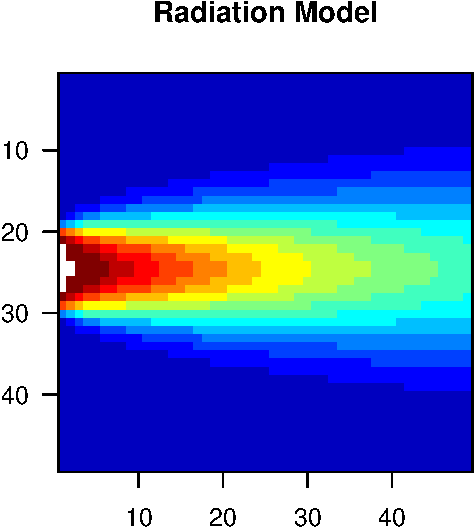
\includegraphics{TumourSurvival_files/figure-latex/unnamed-chunk-1-1} \end{center}

So far so good, we have successfully loaded the data modeling how a beam
of radiation penetrates an area of water. Assuming that living tissue
has similar properties to water, this same model can apply to radiating
tumours.

\subsection{Rotating the Beam}\label{rotating-the-beam}

Now we need to figure out how to rotate the beam an angle \(\theta_1\).
We are going to achieve this by populating a new data frame with the
strength that each point would receive if it were rotated by
\(\theta_1\) radians. This will achieve the same effect as rotating the
beam by -\(\theta_1\) radians.

\begin{Shaded}
\begin{Highlighting}[]
\CommentTok{#First let's tell the computer how many iterations we need to fill the grid}
\NormalTok{iterationsx =}\StringTok{ }\KeywordTok{dim}\NormalTok{(dose)[}\DecValTok{1}\NormalTok{]}
\NormalTok{iterationsy =}\StringTok{ }\KeywordTok{dim}\NormalTok{(dose)[}\DecValTok{2}\NormalTok{]}
\CommentTok{#now let's set the angle that we want to rotate the beam}
\NormalTok{theta1 =}\StringTok{ }\OperatorTok{-}\NormalTok{pi}\OperatorTok{/}\DecValTok{3}
\CommentTok{#and define the rotation matrix that will rotate a vector by that amount}
\NormalTok{rotation1 =}\StringTok{ }\KeywordTok{c}\NormalTok{(}\KeywordTok{cos}\NormalTok{(theta1), }\KeywordTok{sin}\NormalTok{(theta1), }\OperatorTok{-}\KeywordTok{sin}\NormalTok{(theta1), }\KeywordTok{cos}\NormalTok{(theta1))}
\NormalTok{A1 =}\StringTok{ }\KeywordTok{matrix}\NormalTok{(rotation1, }\DataTypeTok{nrow =} \DecValTok{2}\NormalTok{, }\DataTypeTok{ncol =} \DecValTok{2}\NormalTok{)}
\CommentTok{#Now let's make an empty grid (its technically a matrix) to populate with the dosage values}
\NormalTok{output1 <-}\StringTok{ }\KeywordTok{matrix}\NormalTok{(}\DataTypeTok{ncol=}\NormalTok{iterationsy, }\DataTypeTok{nrow=}\NormalTok{iterationsx)}
\CommentTok{#And now we can populate that grid with the new dosage values from the rotated beam using a for loop}
\ControlFlowTok{for}\NormalTok{(i }\ControlFlowTok{in} \DecValTok{1}\OperatorTok{:}\NormalTok{iterationsx)\{}
  \ControlFlowTok{for}\NormalTok{(j }\ControlFlowTok{in} \DecValTok{1}\OperatorTok{:}\NormalTok{iterationsy)\{}
\NormalTok{    vec =}\StringTok{ }\KeywordTok{matrix}\NormalTok{(}\KeywordTok{c}\NormalTok{((i}\OperatorTok{-}\DecValTok{25}\NormalTok{),(j}\OperatorTok{-}\DecValTok{25}\NormalTok{)), }\DataTypeTok{nrow =} \DecValTok{2}\NormalTok{, }\DataTypeTok{ncol =} \DecValTok{1}\NormalTok{)}
\NormalTok{    rot =}\StringTok{ }\NormalTok{A1 }\OperatorTok\StringTok{ }\NormalTok{vec}
    \ControlFlowTok{if}\NormalTok{(}\KeywordTok{round}\NormalTok{(rot[}\DecValTok{1}\NormalTok{])}\OperatorTok{<=-}\DecValTok{25}\NormalTok{)\{}
\NormalTok{      output1[i,j] <-}\StringTok{ }\DecValTok{0}
\NormalTok{    \} }\ControlFlowTok{else}\NormalTok{ \{}\ControlFlowTok{if}\NormalTok{(}\KeywordTok{round}\NormalTok{(rot[}\DecValTok{1}\NormalTok{])}\OperatorTok{>=}\DecValTok{25}\NormalTok{)\{}
\NormalTok{      output1[i,j] <-}\StringTok{ }\DecValTok{0}
\NormalTok{    \} }\ControlFlowTok{else}\NormalTok{ \{}\ControlFlowTok{if}\NormalTok{(}\KeywordTok{round}\NormalTok{(rot[}\DecValTok{2}\NormalTok{])}\OperatorTok{>=}\DecValTok{25}\NormalTok{)\{}
\NormalTok{      output1[i,j] <-}\StringTok{ }\DecValTok{0}
\NormalTok{    \} }\ControlFlowTok{else}\NormalTok{ \{}\ControlFlowTok{if}\NormalTok{(}\KeywordTok{round}\NormalTok{(rot[}\DecValTok{2}\NormalTok{])}\OperatorTok{<=-}\DecValTok{25}\NormalTok{)\{}
\NormalTok{      output1[i,j] <-}\StringTok{ }\DecValTok{0}
\NormalTok{    \} }\ControlFlowTok{else}\NormalTok{ \{output1[i,j] <-}\StringTok{ }\NormalTok{dose[(}\KeywordTok{round}\NormalTok{(rot[}\DecValTok{1}\NormalTok{])}\OperatorTok{+}\DecValTok{25}\NormalTok{), (}\KeywordTok{round}\NormalTok{(rot[}\DecValTok{2}\NormalTok{])}\OperatorTok{+}\DecValTok{25}\NormalTok{)]}
\NormalTok{    \}\}}
\NormalTok{    \}}
\NormalTok{    \}}
\NormalTok{  \}}
\NormalTok{\}}

\CommentTok{#And let's take a peek to ensure we rotated the beam and didn't cause complete chaos}
\KeywordTok{imagesc}\NormalTok{(output1, }\DataTypeTok{xlab=}\StringTok{""}\NormalTok{, }\DataTypeTok{ylab=}\StringTok{""}\NormalTok{, }\DataTypeTok{col=}\KeywordTok{jet.colors}\NormalTok{(}\DecValTok{16}\NormalTok{), }\DataTypeTok{main =} \StringTok{"The Beam Rotated by Pi/3 Radians"}\NormalTok{)}
\end{Highlighting}
\end{Shaded}

\begin{center}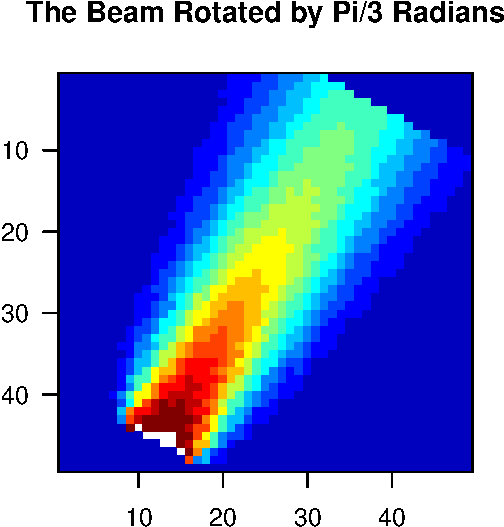
\includegraphics{TumourSurvival_files/figure-latex/unnamed-chunk-2-1} \end{center}

Yay the beam has rotated! Notice however that part of the beam got cut
off when we rotated the square grid. This will be okay as long as the
tumours we consider reside within a distance of 24.5 square widths of
the centre.

If we want to consider multiple beams penetrating from different angles,
say \(\theta_2\) and \(\theta_3\), then we can simply repeat this
process.

\begin{Shaded}
\begin{Highlighting}[]
\CommentTok{#set the angle}
\NormalTok{theta2 =}\StringTok{ }\NormalTok{pi}\OperatorTok{/}\DecValTok{3}
\CommentTok{#define the rotation matrix}
\NormalTok{rotation2 =}\StringTok{ }\KeywordTok{c}\NormalTok{(}\KeywordTok{cos}\NormalTok{(theta2), }\KeywordTok{sin}\NormalTok{(theta2), }\OperatorTok{-}\KeywordTok{sin}\NormalTok{(theta2), }\KeywordTok{cos}\NormalTok{(theta2))}
\NormalTok{A2 =}\StringTok{ }\KeywordTok{matrix}\NormalTok{(rotation2, }\DataTypeTok{nrow =} \DecValTok{2}\NormalTok{, }\DataTypeTok{ncol =} \DecValTok{2}\NormalTok{)}
\CommentTok{#make an empty grid }
\NormalTok{output2 <-}\StringTok{ }\KeywordTok{matrix}\NormalTok{(}\DataTypeTok{ncol=}\NormalTok{iterationsy, }\DataTypeTok{nrow=}\NormalTok{iterationsx)}
\CommentTok{#populate that grid with the new dosage values}
\ControlFlowTok{for}\NormalTok{(i }\ControlFlowTok{in} \DecValTok{1}\OperatorTok{:}\NormalTok{iterationsx)\{}
  \ControlFlowTok{for}\NormalTok{(j }\ControlFlowTok{in} \DecValTok{1}\OperatorTok{:}\NormalTok{iterationsy)\{}
\NormalTok{    vec =}\StringTok{ }\KeywordTok{matrix}\NormalTok{(}\KeywordTok{c}\NormalTok{((i}\OperatorTok{-}\DecValTok{25}\NormalTok{),(j}\OperatorTok{-}\DecValTok{25}\NormalTok{)), }\DataTypeTok{nrow =} \DecValTok{2}\NormalTok{, }\DataTypeTok{ncol =} \DecValTok{1}\NormalTok{)}
\NormalTok{    rot =}\StringTok{ }\NormalTok{A2 }\OperatorTok\StringTok{ }\NormalTok{vec}
    \ControlFlowTok{if}\NormalTok{(}\KeywordTok{round}\NormalTok{(rot[}\DecValTok{1}\NormalTok{])}\OperatorTok{<=-}\DecValTok{25}\NormalTok{)\{}
\NormalTok{      output2[i,j] <-}\StringTok{ }\DecValTok{0}
\NormalTok{    \} }\ControlFlowTok{else}\NormalTok{ \{}\ControlFlowTok{if}\NormalTok{(}\KeywordTok{round}\NormalTok{(rot[}\DecValTok{1}\NormalTok{])}\OperatorTok{>=}\DecValTok{25}\NormalTok{)\{}
\NormalTok{      output2[i,j] <-}\StringTok{ }\DecValTok{0}
\NormalTok{    \} }\ControlFlowTok{else}\NormalTok{ \{}\ControlFlowTok{if}\NormalTok{(}\KeywordTok{round}\NormalTok{(rot[}\DecValTok{2}\NormalTok{])}\OperatorTok{>=}\DecValTok{25}\NormalTok{)\{}
\NormalTok{      output2[i,j] <-}\StringTok{ }\DecValTok{0}
\NormalTok{    \} }\ControlFlowTok{else}\NormalTok{ \{}\ControlFlowTok{if}\NormalTok{(}\KeywordTok{round}\NormalTok{(rot[}\DecValTok{2}\NormalTok{])}\OperatorTok{<=-}\DecValTok{25}\NormalTok{)\{}
\NormalTok{      output2[i,j] <-}\StringTok{ }\DecValTok{0}
\NormalTok{    \} }\ControlFlowTok{else}\NormalTok{ \{output2[i,j] <-}\StringTok{ }\NormalTok{dose[(}\KeywordTok{round}\NormalTok{(rot[}\DecValTok{1}\NormalTok{])}\OperatorTok{+}\DecValTok{25}\NormalTok{), (}\KeywordTok{round}\NormalTok{(rot[}\DecValTok{2}\NormalTok{])}\OperatorTok{+}\DecValTok{25}\NormalTok{)]}
\NormalTok{    \}\}}
\NormalTok{    \}}
\NormalTok{    \}}
\NormalTok{  \}}
\NormalTok{\}}

\CommentTok{#ensure we rotated the beam and didn't cause complete chaos}
\KeywordTok{imagesc}\NormalTok{(output2, }\DataTypeTok{xlab=}\StringTok{""}\NormalTok{, }\DataTypeTok{ylab=}\StringTok{""}\NormalTok{, }\DataTypeTok{col=}\KeywordTok{jet.colors}\NormalTok{(}\DecValTok{16}\NormalTok{), }\DataTypeTok{main =} \StringTok{"The Beam Rotated by -Pi/3 Radians"}\NormalTok{)}
\end{Highlighting}
\end{Shaded}

\begin{center}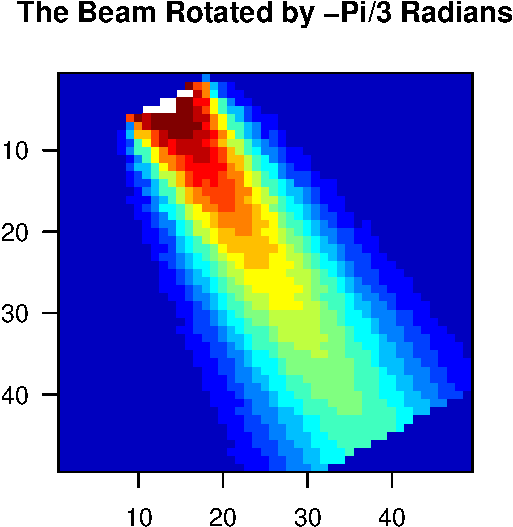
\includegraphics{TumourSurvival_files/figure-latex/unnamed-chunk-3-1} \end{center}

\begin{Shaded}
\begin{Highlighting}[]
\CommentTok{#set the angle}
\NormalTok{theta3 =}\StringTok{ }\OperatorTok{-}\NormalTok{pi}\OperatorTok{/}\DecValTok{58}
\CommentTok{#define the rotation matrix}
\NormalTok{rotation3 =}\StringTok{ }\KeywordTok{c}\NormalTok{(}\KeywordTok{cos}\NormalTok{(theta3), }\KeywordTok{sin}\NormalTok{(theta3), }\OperatorTok{-}\KeywordTok{sin}\NormalTok{(theta3), }\KeywordTok{cos}\NormalTok{(theta3))}
\NormalTok{A3 =}\StringTok{ }\KeywordTok{matrix}\NormalTok{(rotation3, }\DataTypeTok{nrow =} \DecValTok{2}\NormalTok{, }\DataTypeTok{ncol =} \DecValTok{2}\NormalTok{)}
\CommentTok{#make an empty grid}
\NormalTok{output3 <-}\StringTok{ }\KeywordTok{matrix}\NormalTok{(}\DataTypeTok{ncol=}\NormalTok{iterationsy, }\DataTypeTok{nrow=}\NormalTok{iterationsx)}
\CommentTok{#populate that grid}
\ControlFlowTok{for}\NormalTok{(i }\ControlFlowTok{in} \DecValTok{1}\OperatorTok{:}\NormalTok{iterationsx)\{}
  \ControlFlowTok{for}\NormalTok{(j }\ControlFlowTok{in} \DecValTok{1}\OperatorTok{:}\NormalTok{iterationsy)\{}
\NormalTok{    vec =}\StringTok{ }\KeywordTok{matrix}\NormalTok{(}\KeywordTok{c}\NormalTok{((i}\OperatorTok{-}\DecValTok{25}\NormalTok{),(j}\OperatorTok{-}\DecValTok{25}\NormalTok{)), }\DataTypeTok{nrow =} \DecValTok{2}\NormalTok{, }\DataTypeTok{ncol =} \DecValTok{1}\NormalTok{)}
\NormalTok{    rot =}\StringTok{ }\NormalTok{A3 }\OperatorTok\StringTok{ }\NormalTok{vec}
    \ControlFlowTok{if}\NormalTok{(}\KeywordTok{round}\NormalTok{(rot[}\DecValTok{1}\NormalTok{])}\OperatorTok{<=-}\DecValTok{25}\NormalTok{)\{}
\NormalTok{      output3[i,j] <-}\StringTok{ }\DecValTok{0}
\NormalTok{    \} }\ControlFlowTok{else}\NormalTok{ \{}\ControlFlowTok{if}\NormalTok{(}\KeywordTok{round}\NormalTok{(rot[}\DecValTok{1}\NormalTok{])}\OperatorTok{>=}\DecValTok{25}\NormalTok{)\{}
\NormalTok{      output3[i,j] <-}\StringTok{ }\DecValTok{0}
\NormalTok{      \} }\ControlFlowTok{else}\NormalTok{ \{}\ControlFlowTok{if}\NormalTok{(}\KeywordTok{round}\NormalTok{(rot[}\DecValTok{2}\NormalTok{])}\OperatorTok{>=}\DecValTok{25}\NormalTok{)\{}
\NormalTok{        output3[i,j] <-}\StringTok{ }\DecValTok{0}
\NormalTok{      \} }\ControlFlowTok{else}\NormalTok{ \{}\ControlFlowTok{if}\NormalTok{(}\KeywordTok{round}\NormalTok{(rot[}\DecValTok{2}\NormalTok{])}\OperatorTok{<=-}\DecValTok{25}\NormalTok{)\{}
\NormalTok{        output3[i,j] <-}\StringTok{ }\DecValTok{0}
\NormalTok{      \} }\ControlFlowTok{else}\NormalTok{ \{output3[i,j] <-}\StringTok{ }\NormalTok{dose[(}\KeywordTok{round}\NormalTok{(rot[}\DecValTok{1}\NormalTok{])}\OperatorTok{+}\DecValTok{25}\NormalTok{), (}\KeywordTok{round}\NormalTok{(rot[}\DecValTok{2}\NormalTok{])}\OperatorTok{+}\DecValTok{25}\NormalTok{)]}
\NormalTok{      \}\}}
\NormalTok{      \}}
\NormalTok{    \}}
\NormalTok{  \}}
\NormalTok{\}}

\CommentTok{#ensure we rotated the beam and didn't cause complete chaos}
\KeywordTok{imagesc}\NormalTok{(output3, }\DataTypeTok{xlab=}\StringTok{""}\NormalTok{, }\DataTypeTok{ylab=}\StringTok{""}\NormalTok{, }\DataTypeTok{col=}\KeywordTok{jet.colors}\NormalTok{(}\DecValTok{16}\NormalTok{), }\DataTypeTok{main =} \StringTok{"The Beam Rotated by Pi/42 Radians"}\NormalTok{)}
\end{Highlighting}
\end{Shaded}

\begin{center}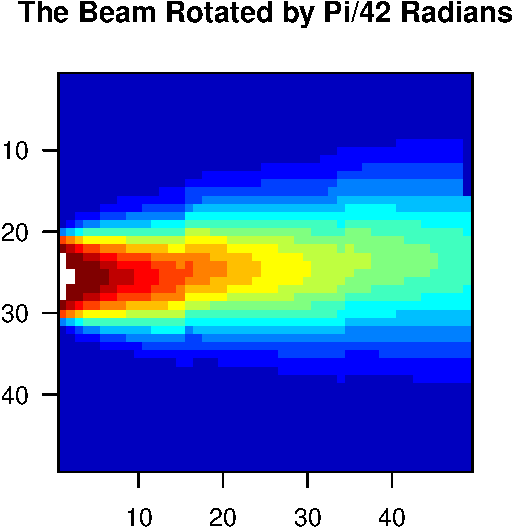
\includegraphics{TumourSurvival_files/figure-latex/unnamed-chunk-3-2} \end{center}

\subsection{Finding the Total Dosage at Each
Point}\label{finding-the-total-dosage-at-each-point}

Now that we have calculated how much radiation each beam deposits at
each point, we can take the sum over the beams to calculate the total
amount of radiation received at each point.

\begin{Shaded}
\begin{Highlighting}[]
\CommentTok{#Let's make a data frame of the total dose received at each  point}
\NormalTok{TotalDose <-}\StringTok{ }\KeywordTok{matrix}\NormalTok{(}\DataTypeTok{ncol=}\NormalTok{iterationsy, }\DataTypeTok{nrow=}\NormalTok{iterationsx)}

\CommentTok{#And now we can populate that grid with the sum of the doses we found above}
\ControlFlowTok{for}\NormalTok{(i }\ControlFlowTok{in} \DecValTok{1}\OperatorTok{:}\NormalTok{iterationsx)\{}
  \ControlFlowTok{for}\NormalTok{(j }\ControlFlowTok{in} \DecValTok{1}\OperatorTok{:}\NormalTok{iterationsy)\{}
\NormalTok{    TotalDose[i,j] <-}\StringTok{ }\NormalTok{output1[i,j]}\OperatorTok{+}\NormalTok{output2[i,j]}\OperatorTok{+}\NormalTok{output3[i,j]}
\NormalTok{        \}}
\NormalTok{\}}
\CommentTok{#make sure that the matrix was populated}
\KeywordTok{imagesc}\NormalTok{(TotalDose, }\DataTypeTok{xlab=}\StringTok{""}\NormalTok{, }\DataTypeTok{ylab=}\StringTok{""}\NormalTok{, }\DataTypeTok{col=}\KeywordTok{jet.colors}\NormalTok{(}\DecValTok{16}\NormalTok{), }\DataTypeTok{main =} \StringTok{"Total Radiation"}\NormalTok{)}
\end{Highlighting}
\end{Shaded}

\begin{center}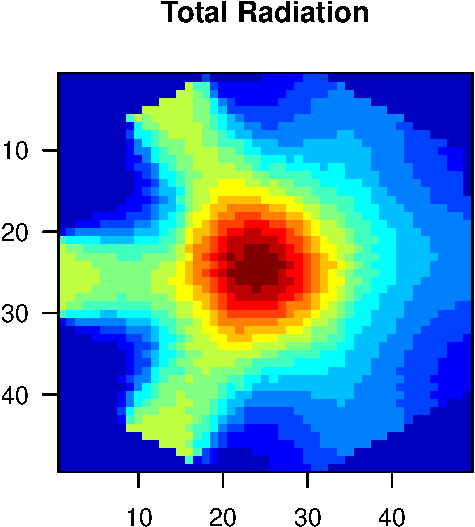
\includegraphics{TumourSurvival_files/figure-latex/unnamed-chunk-4-1} \end{center}

This image shows the total dosage deposited within the region. Recall
that this heat map may not be accurate at points outside a circle of
radius 24.5 since we canculated it by rotating a square of width 49.

\subsection{Time to Introduce a
Tumour}\label{time-to-introduce-a-tumour}

This is all fine and well but we're supposed to be calculating the
amount a tumour survives and so far there's no tumour! Let's fix that
and load a tumour. I generated this tumour by populating a
\(49 \times 49\) grid of zeros in Excel with the value ``1'' in every
cell that I decided would be part of the tumour.

\begin{Shaded}
\begin{Highlighting}[]
\CommentTok{#we need a tumour, so let's load some tumour data}
\NormalTok{Tumour1 <-}\StringTok{ }\KeywordTok{read.csv}\NormalTok{(}\KeywordTok{paste}\NormalTok{(inputlocation, data.files[}\DecValTok{3}\NormalTok{], }\DataTypeTok{sep=}\StringTok{""}\NormalTok{), }\DataTypeTok{stringsAsFactors =} \OtherTok{FALSE}\NormalTok{ )}
\CommentTok{#Let's see what the data looks like}
\KeywordTok{imagesc}\NormalTok{(}\KeywordTok{as.matrix}\NormalTok{(Tumour1), }\DataTypeTok{xlab=}\StringTok{""}\NormalTok{, }\DataTypeTok{ylab=}\StringTok{""}\NormalTok{, }\DataTypeTok{col=}\KeywordTok{jet.colors}\NormalTok{(}\DecValTok{16}\NormalTok{), }\DataTypeTok{main =} \StringTok{"Tumour 1"}\NormalTok{)}
\end{Highlighting}
\end{Shaded}

\begin{center}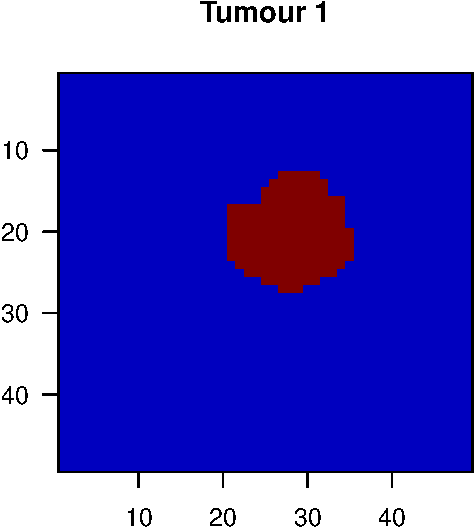
\includegraphics{TumourSurvival_files/figure-latex/unnamed-chunk-5-1} \end{center}

Looks like we successfully loaded the tumour, time to calculate the dose
received at each point.

\begin{Shaded}
\begin{Highlighting}[]
\CommentTok{#Let's make a data frame of the total dose received at each point in the tumour}
\CommentTok{#again, we start with a grid}
\NormalTok{TumourDose1 <-}\StringTok{ }\KeywordTok{matrix}\NormalTok{(}\DataTypeTok{ncol=}\NormalTok{iterationsy, }\DataTypeTok{nrow=}\NormalTok{iterationsx)}

\CommentTok{#And we populate that grid}
\ControlFlowTok{for}\NormalTok{(i }\ControlFlowTok{in} \DecValTok{1}\OperatorTok{:}\NormalTok{iterationsx)\{}
  \ControlFlowTok{for}\NormalTok{(j }\ControlFlowTok{in} \DecValTok{1}\OperatorTok{:}\NormalTok{iterationsy)\{}
\NormalTok{    TumourDose1[i,j] <-}\StringTok{ }\NormalTok{TotalDose[i,j]}\OperatorTok{*}\NormalTok{Tumour1[i,j]}
\NormalTok{  \}}
\NormalTok{\}}

\CommentTok{#take a peek}
\KeywordTok{imagesc}\NormalTok{(TumourDose1, }\DataTypeTok{xlab=}\StringTok{""}\NormalTok{, }\DataTypeTok{ylab=}\StringTok{""}\NormalTok{, }\DataTypeTok{col=}\KeywordTok{jet.colors}\NormalTok{(}\DecValTok{10}\NormalTok{), }\DataTypeTok{main =} \StringTok{"Total Dose Received by Tumour 1"}\NormalTok{)}
\end{Highlighting}
\end{Shaded}

\begin{center}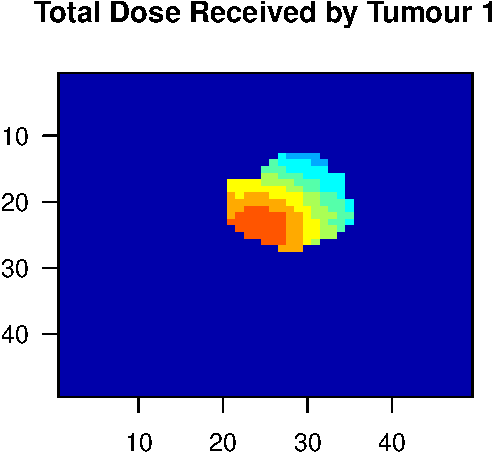
\includegraphics{TumourSurvival_files/figure-latex/unnamed-chunk-6-1} \end{center}

Here we see how much radiation each point in the tumour would
hypothetically receive if it underwent treatment with this beam
configuration. But we aren't done yet! We don't just want to know how
much radiation the tumour gets, we want to know how much of it survives.

\subsection{Calculating the Survival Rate at Each Point in the
Tumour}\label{calculating-the-survival-rate-at-each-point-in-the-tumour}

This is where the Linear Quadratic model defined by McMahon comes in
(McMahon, 2018).The model states,
\[S(p)=e^{-\alpha D(p)-\beta D(p)^2},\] where \(D(p)\) is the dose of
radiation received at point \(p\). This model has parameters \(\alpha\)
and \(\beta\) so let's set those based on the findings in the literature
review by van Leeuwen (van Leeuwen, 2018).

\begin{Shaded}
\begin{Highlighting}[]
\CommentTok{#First we set alpha and beta}
\NormalTok{a =}\StringTok{ }\FloatTok{0.01}
\NormalTok{b =}\StringTok{ }\FloatTok{0.0025}
\end{Highlighting}
\end{Shaded}

Now let's calculate the \(S(p)\) value for each point \(p\) in the
tumour.

\begin{Shaded}
\begin{Highlighting}[]
\CommentTok{#Next we need a data frame of the cell survival}
\NormalTok{CellSurvival1 <-}\StringTok{ }\KeywordTok{matrix}\NormalTok{(}\DataTypeTok{ncol=}\NormalTok{iterationsy, }\DataTypeTok{nrow=}\NormalTok{iterationsx)}

\ControlFlowTok{for}\NormalTok{(i }\ControlFlowTok{in} \DecValTok{1}\OperatorTok{:}\NormalTok{iterationsx)\{}
  \ControlFlowTok{for}\NormalTok{(j }\ControlFlowTok{in} \DecValTok{1}\OperatorTok{:}\NormalTok{iterationsy)\{}
\NormalTok{    CellSurvival1[i,j] <-}\StringTok{ }\KeywordTok{exp}\NormalTok{(}\OperatorTok{-}\NormalTok{(a}\OperatorTok{*}\NormalTok{(TumourDose1[i,j])}\OperatorTok{+}\NormalTok{b}\OperatorTok{*}\NormalTok{(TumourDose1[i,j])}\OperatorTok{^}\DecValTok{2}\NormalTok{))}
\NormalTok{  \}}
\NormalTok{\}}
\CommentTok{#and let's just see how this looks}
\KeywordTok{imagesc}\NormalTok{(CellSurvival1, }\DataTypeTok{xlab=}\StringTok{""}\NormalTok{, }\DataTypeTok{ylab=}\StringTok{""}\NormalTok{, }\DataTypeTok{col=}\KeywordTok{jet.colors}\NormalTok{(}\DecValTok{16}\NormalTok{), }\DataTypeTok{main =} \StringTok{"S(p) of Tumour 1"}\NormalTok{)}
\end{Highlighting}
\end{Shaded}

\begin{center}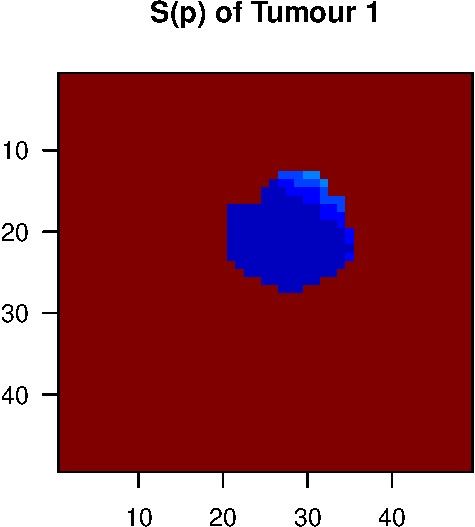
\includegraphics{TumourSurvival_files/figure-latex/unnamed-chunk-8-1} \end{center}

As expected this heat map looks quite similar to the heat map of the
radiation of the tumour, but with the colours inverted. This makes sense
because the points receiving the highest dosage have the lowest survival
rate and vice versa.

\subsection{Quantifying How Much of the Tumour
Survives}\label{quantifying-how-much-of-the-tumour-survives}

At this pont we know the survival rate \(S(p)\) for each gridcell, but
how do we determine how much of the tumour survives? It's a bit tricky
to see with a heat map because there is no scale, so let's make a
histogram to get a sense of how many points in the tumour have any given
\(S(p)\) value.

\begin{Shaded}
\begin{Highlighting}[]
\CommentTok{#First we need to get rid of all the zeros everywhere outside the tumour}
\CommentTok{#because that will throw the histogram off}
\NormalTok{HowZapped1 <-}\StringTok{ }\KeywordTok{matrix}\NormalTok{(}\DataTypeTok{ncol=}\NormalTok{iterationsy, }\DataTypeTok{nrow=}\NormalTok{iterationsx)}
\ControlFlowTok{for}\NormalTok{(i }\ControlFlowTok{in} \DecValTok{1}\OperatorTok{:}\NormalTok{iterationsx)\{}
  \ControlFlowTok{for}\NormalTok{(j }\ControlFlowTok{in} \DecValTok{1}\OperatorTok{:}\NormalTok{iterationsy)\{}
    \ControlFlowTok{if}\NormalTok{(Tumour1[i,j] }\OperatorTok{==}\StringTok{ }\DecValTok{1}\NormalTok{)\{}
\NormalTok{      HowZapped1[i,j] <-}\StringTok{ }\NormalTok{CellSurvival1[i,j]}
\NormalTok{    \} }\ControlFlowTok{else}\NormalTok{ \{}
\NormalTok{      HowZapped1[i,j] <-}\StringTok{ }\OtherTok{NA}\NormalTok{\}}
\NormalTok{  \}}
\NormalTok{\}}
\NormalTok{HowZapped1 <-}\StringTok{ }\KeywordTok{data.frame}\NormalTok{(HowZapped1)}

\CommentTok{#now we can safely create a histogram}
\KeywordTok{hist}\NormalTok{(}\KeywordTok{unlist}\NormalTok{(HowZapped1), }\DataTypeTok{main =} \StringTok{"Histogram of S(p) for Tumour 1"}\NormalTok{, }\DataTypeTok{xlab =} \StringTok{"S(p)"}\NormalTok{, }\DataTypeTok{col =} \StringTok{"red"}\NormalTok{)}
\end{Highlighting}
\end{Shaded}

\begin{center}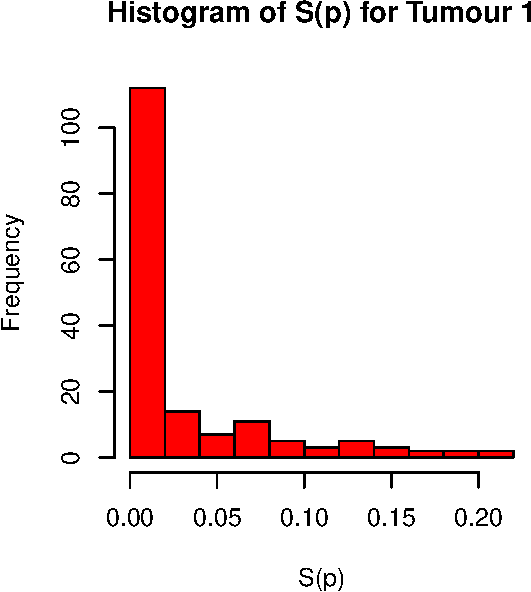
\includegraphics{TumourSurvival_files/figure-latex/unnamed-chunk-9-1} \end{center}

The spike at the low end of this histogram shows that many of the points
in the tumour hve a very low chance of survival, which is good news. At
the other extreme end of the histogram we see that only a small number
of points have a survival rate of over 20\%.

Now that we have calculated \(S(p)\), we can calculate \(SR\), the
metric we have chosen for the amount of the tumour that survives
calculated by, \[SR=\frac{1}{|\Omega|}\sum_{p\in\Omega}S(p),\] where
\(\Omega\) is the size of the tumour, in this case, the number of
gridcells in the tumour (McMahon, 2018). Let us begin by finding
\(\sum_{p\in\Omega}S(p)\).

\begin{Shaded}
\begin{Highlighting}[]
\CommentTok{#to count the S(p) value at each point, we can use another for loop that adds the S(p) value }
\CommentTok{#of the ijth cell in the grid for every gridcell in the tumour}
\NormalTok{sumSp1 =}\StringTok{ }\DecValTok{0}
\ControlFlowTok{for}\NormalTok{(i }\ControlFlowTok{in} \DecValTok{1}\OperatorTok{:}\NormalTok{iterationsx)\{}
  \ControlFlowTok{for}\NormalTok{(j }\ControlFlowTok{in} \DecValTok{1}\OperatorTok{:}\NormalTok{iterationsy)\{}
    \ControlFlowTok{if}\NormalTok{(Tumour1[i,j] }\OperatorTok{==}\StringTok{ }\DecValTok{1}\NormalTok{)\{}
\NormalTok{      sumSp1 <-}\StringTok{ }\NormalTok{sumSp1}\OperatorTok{+}\NormalTok{CellSurvival1[i,j]}
\NormalTok{    \}}
\NormalTok{    \}}
\NormalTok{\}}

\NormalTok{sumSp1}
\end{Highlighting}
\end{Shaded}

\begin{verbatim}
## [1] 4.985355
\end{verbatim}

Now that we have found \(\sum_{p\in\Omega}S(p)\approx 4.9854\), we need
to calculate \(\Omega\) to get \(SR\).

\begin{Shaded}
\begin{Highlighting}[]
\CommentTok{#we can quantify the size of the original tumour by counting its cells}
\NormalTok{totcells1 =}\StringTok{ }\DecValTok{0}
\ControlFlowTok{for}\NormalTok{(i }\ControlFlowTok{in} \DecValTok{1}\OperatorTok{:}\NormalTok{iterationsx)\{}
  \ControlFlowTok{for}\NormalTok{(j }\ControlFlowTok{in} \DecValTok{1}\OperatorTok{:}\NormalTok{iterationsy)\{}
    \ControlFlowTok{if}\NormalTok{(Tumour1[i,j] }\OperatorTok{==}\StringTok{ }\DecValTok{1}\NormalTok{)\{}
\NormalTok{      totcells1 <-}\StringTok{ }\NormalTok{totcells1}\OperatorTok{+}\DecValTok{1}
\NormalTok{    \}}
\NormalTok{  \}}
\NormalTok{\}}
\CommentTok{#check the number}
\NormalTok{totcells1}
\end{Highlighting}
\end{Shaded}

\begin{verbatim}
## [1] 166
\end{verbatim}

Now we have enough information to calculate \(SR\).

\begin{Shaded}
\begin{Highlighting}[]
\NormalTok{SR1 =}\StringTok{ }\NormalTok{sumSp1}\OperatorTok{/}\NormalTok{totcells1}
\NormalTok{SR1}
\end{Highlighting}
\end{Shaded}

\begin{verbatim}
## [1] 0.03003226
\end{verbatim}

Thus, \(SR\approx 0.030032\), meaning that on average any given point in
the tumour has about a 3.0032 \% chance of surviving the treatment. How
does this compare to other tumours? We can replicate this code for
another one to find out.

\begin{Shaded}
\begin{Highlighting}[]
\CommentTok{#To do so we need a new tumour}
\NormalTok{Tumour2 <-}\StringTok{ }\KeywordTok{read.csv}\NormalTok{(}\KeywordTok{paste}\NormalTok{(inputlocation, data.files[}\DecValTok{4}\NormalTok{], }\DataTypeTok{sep=}\StringTok{""}\NormalTok{), }\DataTypeTok{stringsAsFactors =} \OtherTok{FALSE}\NormalTok{ )}
\CommentTok{#Let's see what the data looks like}
\KeywordTok{imagesc}\NormalTok{(}\KeywordTok{as.matrix}\NormalTok{(Tumour2), }\DataTypeTok{xlab=}\StringTok{""}\NormalTok{, }\DataTypeTok{ylab=}\StringTok{""}\NormalTok{, }\DataTypeTok{col=}\KeywordTok{jet.colors}\NormalTok{(}\DecValTok{16}\NormalTok{), }\DataTypeTok{main =} \StringTok{"Tumour 2"}\NormalTok{)}
\end{Highlighting}
\end{Shaded}

\begin{center}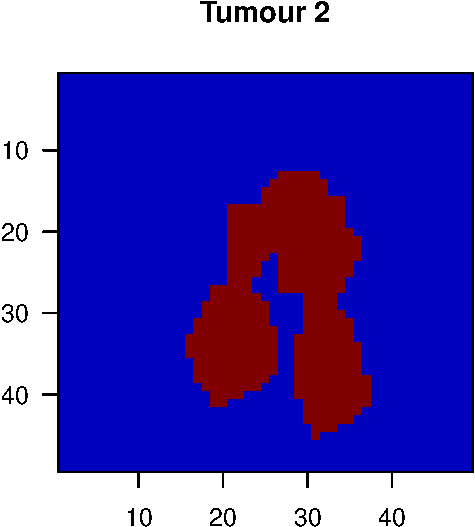
\includegraphics{TumourSurvival_files/figure-latex/unnamed-chunk-13-1} \end{center}

\begin{Shaded}
\begin{Highlighting}[]
\CommentTok{#looks good}

\CommentTok{#Let's make a data frame of the total dose received at each point in the tumour}
\NormalTok{TumourDose2 <-}\StringTok{ }\KeywordTok{matrix}\NormalTok{(}\DataTypeTok{ncol=}\NormalTok{iterationsy, }\DataTypeTok{nrow=}\NormalTok{iterationsx)}

\CommentTok{#And now we can populate that grid}
\ControlFlowTok{for}\NormalTok{(i }\ControlFlowTok{in} \DecValTok{1}\OperatorTok{:}\NormalTok{iterationsx)\{}
  \ControlFlowTok{for}\NormalTok{(j }\ControlFlowTok{in} \DecValTok{1}\OperatorTok{:}\NormalTok{iterationsy)\{}
\NormalTok{    TumourDose2[i,j] <-}\StringTok{ }\NormalTok{TotalDose[i,j]}\OperatorTok{*}\NormalTok{Tumour2[i,j]}
\NormalTok{  \}}
\NormalTok{\}}
\CommentTok{#check it out}
\KeywordTok{imagesc}\NormalTok{(TumourDose2, }\DataTypeTok{xlab=}\StringTok{""}\NormalTok{, }\DataTypeTok{ylab=}\StringTok{""}\NormalTok{, }\DataTypeTok{col=}\KeywordTok{jet.colors}\NormalTok{(}\DecValTok{16}\NormalTok{), }\DataTypeTok{main =} \StringTok{"Total Dosage of Tumour 2"}\NormalTok{)}
\end{Highlighting}
\end{Shaded}

\begin{center}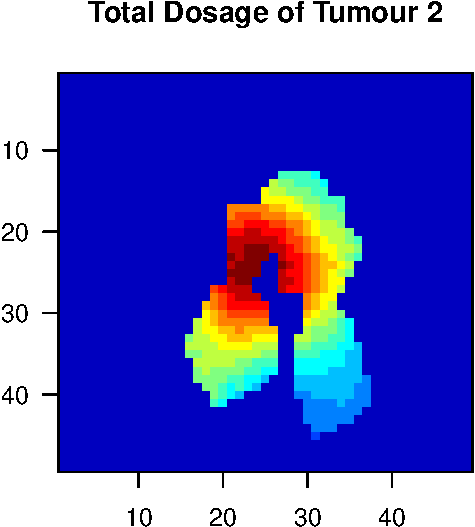
\includegraphics{TumourSurvival_files/figure-latex/unnamed-chunk-13-2} \end{center}

\begin{Shaded}
\begin{Highlighting}[]
\CommentTok{#Let's make a data frame of the cell survival}
\NormalTok{CellSurvival2 <-}\StringTok{ }\KeywordTok{matrix}\NormalTok{(}\DataTypeTok{ncol=}\NormalTok{iterationsy, }\DataTypeTok{nrow=}\NormalTok{iterationsx)}

\CommentTok{#And now we can populate that grid}
\ControlFlowTok{for}\NormalTok{(i }\ControlFlowTok{in} \DecValTok{1}\OperatorTok{:}\NormalTok{iterationsx)\{}
  \ControlFlowTok{for}\NormalTok{(j }\ControlFlowTok{in} \DecValTok{1}\OperatorTok{:}\NormalTok{iterationsy)\{}
\NormalTok{    CellSurvival2[i,j] <-}\StringTok{ }\KeywordTok{exp}\NormalTok{(}\OperatorTok{-}\NormalTok{(a}\OperatorTok{*}\NormalTok{(TumourDose2[i,j])}\OperatorTok{+}\NormalTok{b}\OperatorTok{*}\NormalTok{(TumourDose2[i,j])}\OperatorTok{^}\DecValTok{2}\NormalTok{))}
\NormalTok{  \}}
\NormalTok{\}}

\CommentTok{#visualize}
\KeywordTok{imagesc}\NormalTok{(CellSurvival2, }\DataTypeTok{xlab=}\StringTok{""}\NormalTok{, }\DataTypeTok{ylab=}\StringTok{""}\NormalTok{, }\DataTypeTok{col=}\KeywordTok{jet.colors}\NormalTok{(}\DecValTok{16}\NormalTok{), }\DataTypeTok{main =} \StringTok{"S(p) of Tumour 2"}\NormalTok{)}
\end{Highlighting}
\end{Shaded}

\begin{center}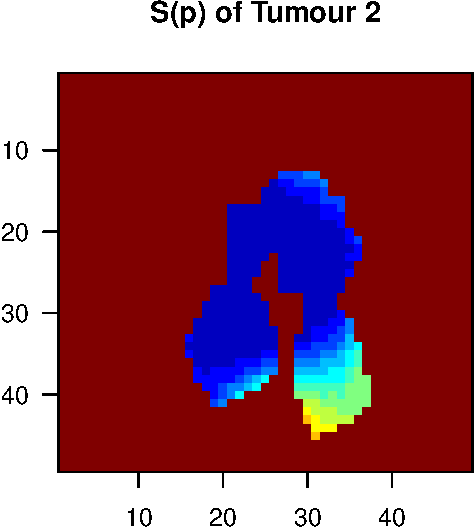
\includegraphics{TumourSurvival_files/figure-latex/unnamed-chunk-13-3} \end{center}

\begin{Shaded}
\begin{Highlighting}[]
\CommentTok{#Now let's make a histogram' to visualize how zapped the tumour was}
\CommentTok{#Get rid of unecessary the zeros}
\NormalTok{HowZapped2 <-}\StringTok{ }\KeywordTok{matrix}\NormalTok{(}\DataTypeTok{ncol=}\NormalTok{iterationsy, }\DataTypeTok{nrow=}\NormalTok{iterationsx)}
\ControlFlowTok{for}\NormalTok{(i }\ControlFlowTok{in} \DecValTok{1}\OperatorTok{:}\NormalTok{iterationsx)\{}
  \ControlFlowTok{for}\NormalTok{(j }\ControlFlowTok{in} \DecValTok{1}\OperatorTok{:}\NormalTok{iterationsy)\{}
    \ControlFlowTok{if}\NormalTok{(TumourDose2[i,j]}\OperatorTok{>}\DecValTok{1}\NormalTok{)\{}
\NormalTok{      HowZapped2[i,j] <-}\StringTok{ }\NormalTok{CellSurvival2[i,j]}
\NormalTok{    \} }\ControlFlowTok{else}\NormalTok{ \{}
\NormalTok{      HowZapped2[i,j] <-}\StringTok{ }\OtherTok{NA}\NormalTok{\}}
\NormalTok{  \}}
\NormalTok{\}}
\NormalTok{HowZapped2 <-}\StringTok{ }\KeywordTok{data.frame}\NormalTok{(HowZapped2)}

\KeywordTok{hist}\NormalTok{(}\KeywordTok{unlist}\NormalTok{(HowZapped2), }\DataTypeTok{main =} \StringTok{"Histogram of S(p) for Tumour  2"}\NormalTok{, }\DataTypeTok{xlab =} \StringTok{"S(p)"}\NormalTok{, }\DataTypeTok{col =} \StringTok{"red"}\NormalTok{)}
\end{Highlighting}
\end{Shaded}

\begin{center}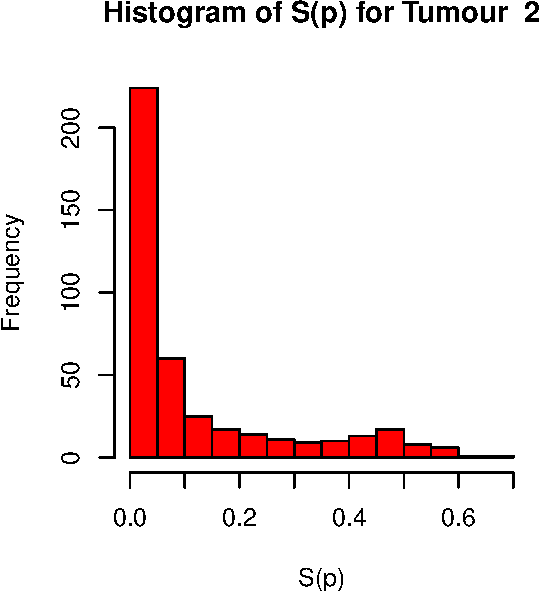
\includegraphics{TumourSurvival_files/figure-latex/unnamed-chunk-13-4} \end{center}

\begin{Shaded}
\begin{Highlighting}[]
\CommentTok{#to count the sum of S(p) over tumour 2 }
\NormalTok{sumSp2 =}\StringTok{ }\DecValTok{0}
\ControlFlowTok{for}\NormalTok{(i }\ControlFlowTok{in} \DecValTok{1}\OperatorTok{:}\NormalTok{iterationsx)\{}
  \ControlFlowTok{for}\NormalTok{(j }\ControlFlowTok{in} \DecValTok{1}\OperatorTok{:}\NormalTok{iterationsy)\{}
    \ControlFlowTok{if}\NormalTok{(Tumour1[i,j] }\OperatorTok{==}\StringTok{ }\DecValTok{1}\NormalTok{)\{}
\NormalTok{      sumSp2 <-}\StringTok{ }\NormalTok{sumSp2}\OperatorTok{+}\NormalTok{CellSurvival2[i,j]}
\NormalTok{    \}}
\NormalTok{    \}}
\NormalTok{\}}
\CommentTok{#let's see how many we got!}
\NormalTok{sumSp2}
\end{Highlighting}
\end{Shaded}

\begin{verbatim}
## [1] 11.98496
\end{verbatim}

\begin{Shaded}
\begin{Highlighting}[]
\CommentTok{#now let's calculate the percentage of the tumour that survived}
\CommentTok{#to do so we need  to quantify the size  of the original tumour}
\NormalTok{totcells2 =}\StringTok{ }\DecValTok{0}
\ControlFlowTok{for}\NormalTok{(i }\ControlFlowTok{in} \DecValTok{1}\OperatorTok{:}\NormalTok{iterationsx)\{}
  \ControlFlowTok{for}\NormalTok{(j }\ControlFlowTok{in} \DecValTok{1}\OperatorTok{:}\NormalTok{iterationsy)\{}
    \ControlFlowTok{if}\NormalTok{(Tumour2[i,j] }\OperatorTok{==}\StringTok{ }\DecValTok{1}\NormalTok{)\{}
\NormalTok{      totcells2 <-}\StringTok{ }\NormalTok{totcells2}\OperatorTok{+}\DecValTok{1}
\NormalTok{    \}}
\NormalTok{  \}}
\NormalTok{\}}
\NormalTok{totcells2}
\end{Highlighting}
\end{Shaded}

\begin{verbatim}
## [1] 416
\end{verbatim}

\begin{Shaded}
\begin{Highlighting}[]
\NormalTok{SR2 =}\StringTok{ }\NormalTok{sumSp2}\OperatorTok{/}\NormalTok{totcells2}
\NormalTok{SR2}
\end{Highlighting}
\end{Shaded}

\begin{verbatim}
## [1] 0.02881
\end{verbatim}

In this case, the expected survival rate at any given point in the
tumour iss about 2.8810 \%. Surprisingly, despide haveing some parts of
the second tumour receive lower doses than any part of the first tumour
received, the \(SR\) value for Tumour 2 is lower than that of Tumour 1
indicating that, by this metric, it has a lower survival rate. Thus, we
caution the reader that although \(SR\) may be a convenient general
metric it may be misleading for tumours where some parts are
over-radiated and others are under-radiated.

\subsection{Works Cited}\label{works-cited}

R. Barnard, M. Frank, M. Herty, ``Optimal radiotherapy treatment
planning using minimum entropy models,'' Applied Mathematics and
Computation, 2012

C.M. van Leeuwen, A.L. Oei, J. Crezee, \textit{et al.} The alfa and beta
of tumours: a review of parameters of the linear-quadratic model,
derived from clinical radiotherapy studies. \textit{Radiat Oncol}
\textbf{13,} 96 (2018).
\href{https://doi.org/10.1186/s13014-018-1040-z}{https://doi.org/10.1186/s13014-018-1040-z}

S. J. McMahon, ``The linear quadratic model: usage, interpretation and
challenges," Physics in Medicine \& Biology, (2018).
\href{https://iopscience.iop.org/article/10.1088/1361-6560/aaf26a}{https://iopscience.iop.org/article/10.1088/1361-6560/aaf26a}

``The Science Behind Radiation Therapy," American Cancer Society,
(2014).
\href{https://www.cancer.org/content/dam/CRC/PDF/Public/6151.00.pdf}{https://www.cancer.org/content/dam/CRC/PDF/Public/6151.00.pdf}


\end{document}
